\documentclass[12pt,a4paper]{article}
\usepackage[utf8]{inputenc}
\usepackage[T1]{fontenc}
\usepackage[brazilian]{babel}
\usepackage{lmodern}
\usepackage[a4paper,margin=2.5cm]{geometry}
\usepackage{booktabs,longtable,array}
\usepackage{amsmath}
\usepackage{graphicx,pdflscape}
\usepackage[hidelinks]{hyperref}
\usepackage{microtype}
\setlength{\emergencystretch}{2em}
\renewcommand{\arraystretch}{1.15}
\newcolumntype{L}[1]{>{\raggedright\arraybackslash}p{#1}}

\title{Projeto de Videogame Portátil com ESP32-S3\\\large Componentes, arquitetura e conexões elétricas}
\author{Isaac da Cunha Cavalcanti Duarti \\ Jhonny Cunha Simões \\ João Pedro Moreira Campos de Lima}
\date{Ciência da Computação -- IFCE Campus Maracanaú\\Disciplina de Microcontroladores\\\today}

\begin{document}
\maketitle
\begin{abstract}
  Este relatório apresenta um videogame portátil baseado no ESP32-S3 N16R8, com display TFT de 2,8 polegadas, armazenamento em cartão SD, oito botões e reprodução de áudio. O sistema é alimentado por uma bateria de lítio de 3,7 V e 1000 mAh, associada a um carregador TP4056, um conversor elevador MT3608 e uma chave liga/desliga. São descritos os componentes, suas funções, a distribuição da alimentação e o mapeamento das interfaces digitais. A documentação elétrica e física do projeto é desenvolvida no KiCad, por meio do esquemático, das bibliotecas de componentes e do layout da placa de circuito impresso.
\end{abstract}

\section{Introdução e objetivo}
O projeto consiste em um console portátil e recarregável destinado à execução de um jogo desenvolvido pela equipe. O ESP32-S3 concentra o processamento: recebe os comandos do usuário, atualiza o estado do jogo, controla a apresentação gráfica e transmite os dados de áudio. A tela apresenta os elementos visuais, enquanto o alto-falante reproduz efeitos sonoros e músicas. O cartão SD oferece armazenamento removível para os recursos utilizados pelo sistema.

A entrada dos comandos do jogo ocorre por oito botões físicos. A bateria fornece autonomia em relação à rede elétrica, e o carregador permite a recarga por USB. A chave SW9 atua no caminho de alimentação dos circuitos do videogame, enquanto SW10 habilita ou desliga internamente o amplificador.

\section{Componentes e funções}
\subsection{ESP32-S3 N16R8}
Placa de desenvolvimento com módulo ESP32-S3, 16 MB de flash e 8 MB de PSRAM. É responsável pelo processamento do jogo e pelas interfaces de entrada, vídeo, armazenamento e áudio.

\subsection{Tela TFT de 2,8 polegadas}
Módulo de exibição com comunicação SPI, interface de touch e conector para cartão SD. A tela constitui a saída gráfica do console; o touch permanece sem conexão externa.

\subsection{Cartão SD}
Memória removível para imagens, mapas, músicas e outros arquivos. Utiliza o conector integrado ao módulo da tela, com sinais SPI separados dos utilizados pelo display.

\subsection{Amplificador MAX98357}
Amplificador digital classe D que recebe dados de áudio e fornece o sinal de potência para o alto-falante.

\subsection{Alto-falante}
Transdutor identificado no esquemático como 8 $\Omega$ e potência nominal de 1 W. Converte o sinal elétrico amplificado em som.

\subsection{Bateria}
Célula de lítio de 3,7 V nominais e capacidade de 1000 mAh, utilizada como fonte de energia portátil.

\subsection{Carregador TP4056}
Módulo de recarga de uma célula de lítio a partir da entrada USB. Possui terminais para a bateria e para a alimentação da carga.

\subsection{Conversor de tensão MT3608}
Conversor CC--CC elevador, responsável pelo barramento de 5 V a partir da tensão da bateria.

\subsection{Indicador de bateria}
Indicador visual de nível da bateria, conectado ao nó de alimentação anterior ao conversor elevador.

\subsection{SW1 a SW8}
Botões momentâneos conectados individualmente aos GPIOs do ESP32-S3, com retorno ao GND.

\subsection{SW9}
Chave SPDT utilizada como liga/desliga, com um contato sem conexão. Interrompe o positivo da alimentação do conversor e do indicador.

\subsection{SW10}
Chave SPDT que conecta o terminal SD/MODE do MAX98357 a 3,3 V ou ao GND, habilitando ou desligando internamente o amplificador. O controle não utiliza um GPIO do ESP32-S3.

\subsection{Processamento e memória}
O ESP32-S3 integra processamento e periféricos de comunicação para sistemas embarcados~\cite{s3}. Na variante N16R8, os 16 MB de flash armazenam o programa e dados persistentes, enquanto os 8 MB de PSRAM ampliam a memória de trabalho disponível para recursos como buffers gráficos e de áudio~\cite{wroom}. O cartão SD complementa essas memórias com armazenamento removível.

As conexões externas do ESP32-S3 distribuem-se entre as interfaces SPI e de áudio digital e as entradas dos botões. Os GPIOs 35, 36 e 37 não possuem conexões externas no esquemático, em correspondência com o uso de PSRAM octal no módulo. Os GPIOs 19 e 20, associados à USB nativa do ESP32-S3, também permanecem sem ligação aos periféricos do console~\cite{s3,wroom}. O GPIO11 permanece sem conexão externa, pois a habilitação do amplificador é realizada por SW10.

\subsection{Arquitetura funcional}
\begin{center}
  \fbox{
    \begin{minipage}{0.91\linewidth}
      \centering
      Botões $\longrightarrow$ GPIOs $\longrightarrow$ ESP32-S3\\[5pt]
      ESP32-S3 $\xrightarrow{\mathrm{SPI\ separado}}$ TFT e cartão SD\\[5pt]
      ESP32-S3 $\xrightarrow{\text{áudio digital}}$ MAX98357 $\longrightarrow$ falante
  \end{minipage}}
\end{center}
O sistema reúne entrada, processamento, saída gráfica, saída sonora e armazenamento. O display e o cartão SD utilizam barramentos SPI separados, cada um com seus sinais de clock, dados e seleção. O áudio utiliza sinais próprios de comunicação digital, e SW10 controla a habilitação do amplificador.

\section{Alimentação e recarga}
\subsection{Distribuição de energia}
A alimentação parte da bateria e alcança os demais circuitos por meio dos terminais de saída do módulo carregador e da chave SW9. O conversor de tensão eleva a tensão para o barramento de 5 V. A placa de desenvolvimento ESP32-S3 recebe esse barramento em sua entrada 5V e dispõe de alimentação regulada de 3,3 V.
\begin{center}
  \fbox{
    \begin{minipage}{0.91\linewidth}
      \centering
      USB $\longrightarrow$ TP4056 $\longleftrightarrow$ bateria\\[5pt]
      OUT+ do carregador $\longrightarrow$ SW9 $\longrightarrow$ MT3608\\[5pt]
      MT3608: 5 V $\longrightarrow$ ESP32-S3, TFT e amplificador\\[5pt]
      Placa ESP32-S3: 3,3 V $\longrightarrow$ LED do TFT e contato 3 de SW10
  \end{minipage}}
\end{center}

A rede \texttt{+BATT} conecta o positivo da bateria ao terminal B+ do carregador, e a rede \texttt{-BATT} conecta seu negativo a B--. Os terminais OUT+ e OUT-- constituem a conexão da carga ao módulo. OUT-- estabelece o GND do console, compartilhado pelo conversor, ESP32-S3, tela, amplificador, indicador e botões.

As redes B-- e OUT-- são distintas no esquemático. Essa separação é característica da conexão externa de módulos que realizam a proteção pelo caminho negativo da bateria. A função de carregamento pertence ao TP4056; funções de proteção contra descarga excessiva e curto-circuito dependem dos circuitos adicionais presentes no módulo ou na bateria.

\subsection{Chave liga/desliga e indicador}
O terminal comum 2 de SW9 conecta-se a OUT+ do carregador TP4056, pino 1. O contato 3 conecta-se a VIN+ do MT3608, pino 3, e a BAT+ do indicador de bateria, pino 2, enquanto o contato 1 permanece sem conexão. A ligação entre 2 e 3 alimenta o conversor e o indicador; a posição entre 2 e 1 interrompe esse caminho. O terminal BAT-- do indicador, pino 1, está ligado ao GND.

A chave atua sobre a carga, mantendo a conexão entre bateria e carregador. Dessa forma, a bateria pode ser recarregada com os circuitos do console desligados. O indicador acompanha a tensão disponível antes da elevação para 5 V, fornecendo uma indicação aproximada do nível de carga.

\subsection{Conversão de tensão}
O MT3608 é um conversor elevador de tensão~\cite{mt}. No projeto, VIN+ recebe a alimentação comutada da bateria, VIN-- e VOUT-- estão ligados ao GND e VOUT+ pertence à rede \texttt{+5V}. Essa rede alimenta o ESP32-S3, o VCC do display e o VIN do amplificador.

A elevação de tensão implica uma corrente de entrada superior à corrente fornecida na saída, considerando a mesma potência e as perdas de conversão. Para rendimento $\eta$, tensão de bateria $V_{\mathrm{bat}}$ e corrente total $I_{5V}$:
\[
  I_{\mathrm{bat}}\simeq\frac{5\,I_{5V}}{\eta\,V_{\mathrm{bat}}}.
\]
Como exemplo teórico, uma carga de 0,5 A em 5 V, com bateria em 3,7 V e rendimento de 85\%, corresponde a aproximadamente 0,80 A na entrada. O consumo efetivo varia com a atividade do processador, os acessos ao cartão, a iluminação da tela e a reprodução sonora.

\subsection{Carregamento da bateria}
A entrada USB do módulo TP4056 fornece energia ao circuito de recarga. Os terminais IN+ e IN-- não possuem fios externos no esquemático, pois a alimentação de recarga é realizada pelo conector do próprio módulo.

O TP4056 aplica o processo de corrente constante e tensão constante para uma célula de lítio, com tensão final de 4,2 V na versão documentada. A corrente de carga é estabelecida por um resistor de programação~\cite{tp}. O valor desse resistor não é representado no símbolo do módulo utilizado no projeto.

O carregador é linear, e sua dissipação pode ser aproximada por $P\simeq(V_{\mathrm{USB}}-V_{\mathrm{bat}})I_{\mathrm{carga}}$. Para entrada de 5 V, bateria em 3,7 V e corrente de 0,5 A, essa expressão resulta em 0,65 W. Trata-se de um exemplo teórico de dissipação.

A topologia representada não inclui um circuito dedicado de compartilhamento de alimentação, denominado \textit{power path}. A recarga com SW9 aberta mantém o consumo do console separado do processo de carga. Em carregadores com término por corrente, o consumo simultâneo de uma carga ligada à bateria pode interferir na identificação do final da recarga~\cite{loadsharing}.

\subsection{Energia e autonomia teórica}
A energia nominal da bateria é aproximadamente:
\[
  E_{\mathrm{bat}}=3{,}7\,\mathrm{V}\times1{,}0\,\mathrm{Ah}=3{,}7\,\mathrm{Wh}.
\]
Para um rendimento ilustrativo de 85\% no elevador, a autonomia teórica em horas é:
\[
  t\simeq\frac{3{,}7\times0{,}85}{5\,I_{5V}}.
\]
\begin{center}
  \begin{tabular}{ccc}
    \toprule
    \textbf{Corrente em 5 V} & \textbf{Potência} & \textbf{Autonomia teórica}\\
    \midrule
    0,30 A & 1,50 W & 2,10 h\\
    0,50 A & 2,50 W & 1,26 h\\
    0,70 A & 3,50 W & 0,90 h\\
    \bottomrule
  \end{tabular}
\end{center}
Os valores representam cenários de cálculo, sem medições de consumo do console. A autonomia real depende da capacidade útil da célula, do limite de descarga, da eficiência dos reguladores e do perfil de uso.

\section{Display e armazenamento}
\subsection{Conexões dos barramentos SPI}
O display e o cartão SD utilizam sinais MOSI, MISO e SCK separados. A linha MOSI transporta dados do ESP32-S3 ao periférico; MISO transporta os dados de retorno; e SCK fornece o clock de comunicação. Cada dispositivo possui sua linha de seleção, conforme o mapeamento a seguir. Os dois conjuntos de terminais pertencem ao módulo U4.
\begin{longtable}{@{}L{0.22\linewidth}L{0.12\linewidth}L{0.59\linewidth}@{}}
  \toprule
  \textbf{Rede} & \textbf{GPIO} & \textbf{Destino na tela}\\
  \midrule
  \endhead
  \texttt{TFT\_MOSI} & 18 & SDI (MOSI) do TFT, pino 6.\\
  \texttt{TFT\_MISO} & 16 & SDO (MISO) do TFT, pino 9.\\
  \texttt{TFT\_SCK} & 15 & Clock do TFT, pino 7.\\
  \texttt{TFT\_CS} & 10 & Seleção do TFT, pino 3.\\
  \texttt{TFT\_DC} & 8 & Seleção comando/dado do TFT, pino 5.\\
  \texttt{TFT\_RESET} & 9 & Reset do controlador da tela, pino 4.\\
  \texttt{SD\_MOSI} & 6 & MOSI do cartão SD, pino 16.\\
  \texttt{SD\_MISO} & 5 & MISO do cartão SD, pino 17.\\
  \texttt{SD\_SCK} & 4 & Clock do cartão SD, pino 18.\\
  \texttt{SD\_CS} & 7 & Seleção do cartão SD, pino 15.\\
  \bottomrule
\end{longtable}

A seleção do TFT ocorre pela rede \texttt{TFT\_CS}, ligada ao GPIO10, enquanto a seleção do SD utiliza \texttt{SD\_CS}, ligada ao GPIO7. As seleções são ativas em nível baixo. As linhas MISO também são independentes: GPIO16 para o TFT e GPIO5 para o SD.

O sinal DC distingue comandos de dados enviados ao controlador gráfico. RESET controla a reinicialização do display por um GPIO próprio, sem conexão ao reset geral da placa ESP32-S3. A escolha de GPIOs para SPI utiliza os recursos de roteamento dos sinais periféricos do microcontrolador~\cite{s3}.

\subsection{Alimentação da tela e interface de touch}
O VCC da tela, pino 1, está ligado ao barramento de 5 V. O terminal LED, pino 8, está ligado à rede de 3,3 V da placa ESP32-S3, e o pino 2 está conectado ao GND. VCC corresponde à alimentação do módulo, enquanto LED é o terminal associado à iluminação da tela. As tensões dessas redes são distintas dos níveis lógicos de comunicação do ESP32-S3, que utiliza sinais de 3,3 V.

O esquemático identifica o módulo como TFT de 2,8 polegadas com touch. O símbolo apresenta seus terminais externos, sem especificar o controlador gráfico, a resolução ou o circuito interno de alimentação e iluminação.

Os sinais T\_CLK, T\_CS, T\_DIN, T\_DO e T\_IRQ, correspondentes aos pinos 10 a 14, permanecem sem ligação externa. Portanto, a interface de touch não participa da entrada de comandos. Os terminais SD\_CS, SD\_MOSI, SD\_MISO e SD\_SCK correspondem à interface do cartão de memória integrado ao módulo.

\section{Subsistema de áudio}
O áudio é transmitido do ESP32-S3 ao módulo MAX98357 por três sinais: DIN transporta as amostras, BCLK determina o ritmo dos bits e LRC identifica os canais e a cadência das amostras.
\begin{center}
  \begin{tabular}{lll}
    \toprule
    \textbf{Rede} & \textbf{GPIO} & \textbf{Destino no amplificador}\\
    \midrule
    \texttt{DIN} & 12 & DIN, pino 3\\
    \texttt{BCLK} & 13 & BCLK, pino 2\\
    \texttt{LRC} & 14 & LRC/LRCLK, pino 1\\
    \bottomrule
  \end{tabular}
\end{center}

O MAX98357A recebe áudio no formato I\textsuperscript{2}S e não exige clock mestre MCLK. O MAX98357B utiliza o formato justificado à esquerda~\cite{max}. No esquemático, o amplificador recebe 5 V em VIN, pino 7, e sua referência de terra é estabelecida pelo pino 6.

O terminal GAIN, pino 4, permanece sem conexão externa, e sua configuração depende dos componentes presentes no módulo. O terminal SD/MODE, pino 5, pertence à rede \texttt{AMP\_SD}, ligada exclusivamente ao terminal comum 2 de SW10. O GPIO11 não participa dessa rede.

\subsection{Chave de áudio SW10}
\begin{center}
  \begin{tabular}{lll}
    \toprule
    \textbf{Terminal de SW10} & \textbf{Rede} & \textbf{Destino}\\
    \midrule
    1 & GND & Terra comum\\
    2 (comum) & \texttt{AMP\_SD} & SD/MODE de U7, pino 5\\
    3 & 3V3 & Saída de 3,3 V de U1, pino 1\\
    \bottomrule
  \end{tabular}
\end{center}
A ligação entre 2 e 3 aplica 3,3 V ao SD/MODE e habilita o amplificador, selecionando o canal esquerdo. A ligação entre 2 e 1 aplica GND e coloca o amplificador em desligamento interno~\cite{max}. A chave não interrompe o VIN de 5 V; o ESP32-S3 e a tela continuam alimentados. Não há resistor externo nessa ligação. A chave física deve desconectar um contato antes de conectar o outro, e seu terminal comum deve ser identificado conforme o modelo utilizado.

O alto-falante LS1 está identificado no esquemático com impedância nominal de 8 $\Omega$ e potência de 1 W. Sua ligação é prevista diretamente no borne do módulo, com fios fixados por parafusos. Os dois pinos de LS1 estão marcados como sem conexão no desenho, acompanhados dessa indicação de montagem. O símbolo do amplificador representa os terminais de alimentação e entrada; o borne de saída não está incluído nessa representação.

A saída para o falante é diferencial, entre os dois terminais do amplificador~\cite{max}. A relação entre potência, impedância e tensão eficaz diferencial é $P=V_{\mathrm{ef}}^2/R$. Para 1 W em 8 $\Omega$, essa relação corresponde a aproximadamente 2,83 V eficazes em um sinal senoidal.

\section{Controles físicos}
Cada botão conecta um GPIO ao GND quando pressionado. O uso de sinais individuais permite a identificação independente dos oito comandos, sem uma matriz de varredura. O mapeamento é apresentado a seguir.
\begin{center}
  \begin{tabular}{llll}
    \toprule
    \textbf{Botão} & \textbf{Rede} & \textbf{GPIO} & \textbf{Outro terminal}\\
    \midrule
    SW1 & Button-1 & 2 & GND\\
    SW2 & Button-2 & 42 & GND\\
    SW3 & Button-3 & 41 & GND\\
    SW4 & Button-4 & 39 & GND\\
    SW5 & Button-5 & 40 & GND\\
    SW6 & Button-6 & 38 & GND\\
    SW7 & Button-7 & 21 & GND\\
    SW8 & Button-8 & 47 & GND\\
    \bottomrule
  \end{tabular}
\end{center}

O GPIO48 está ligado ao LED RGB integrado à placa de desenvolvimento, conforme confirmado por teste de alternância entre vermelho, verde, azul e apagado. Esse pino permanece sem conexão externa no projeto. A distribuição dos botões foi reorganizada para liberar o GPIO48 e acompanhar a sequência das trilhas na PCB.

A lógica de leitura é ativa em nível baixo: com entrada polarizada por \textit{pull-up}, o botão solto corresponde ao nível 1 e o botão pressionado corresponde ao nível 0. O esquema não apresenta resistores externos de polarização para os botões; o ESP32-S3 dispõe de \textit{pull-ups} internos configuráveis~\cite{s3}.

Os contatos mecânicos podem apresentar transições breves durante o acionamento, fenômeno conhecido como repique ou \textit{bounce}. O tratamento desse efeito permite interpretar um acionamento físico como um único comando. A associação dos oito botões às ações do jogo é definida pela lógica da aplicação.

\section{Documentação e placa de circuito impresso}
O projeto utiliza o KiCad para representar as conexões e a disposição física dos componentes. O arquivo \texttt{playboyzinho.kicad\_sch} contém o esquemático, e \texttt{playboyzinho.kicad\_pcb} contém o layout da placa. A biblioteca \texttt{lib-do-playboy.kicad\_sym} e os footprints de \texttt{lib-do-playboy.pretty} representam os módulos e suas interfaces de montagem.

O arquivo da PCB define uma placa com espessura nominal de 1,6 mm, material dielétrico FR4 e duas camadas de cobre, F.Cu e B.Cu. Os footprints correspondem aos módulos de alimentação, processamento, display, áudio e indicador, além dos botões, da chave e da conexão da bateria. Essa estrutura reúne os subsistemas em uma base de interligação física.

As referências dos componentes relacionam os elementos do esquemático aos seus footprints. Os rótulos de rede identificam conexões como \texttt{TFT\_MOSI}, \texttt{SD\_SCK}, \texttt{AMP\_SD}, \texttt{DIN} e \texttt{Button-1}, inclusive quando os trechos correspondentes aparecem afastados no desenho. Os símbolos \texttt{PWR\_FLAG} são elementos de documentação elétrica do KiCad associados à indicação de redes alimentadas, sem componente físico correspondente.

\section{Funcionamento do console}
Ao fechar SW9, a alimentação da bateria alcança o conversor elevador e o indicador. O barramento de 5 V alimenta a placa ESP32-S3, a tela e o amplificador. Durante a operação, o processador lê os botões, executa a lógica do jogo, acessa recursos no cartão SD e apresenta as saídas gráficas e sonoras.

A comunicação com a tela e o cartão ocorre por barramentos SPI separados, com seleção individual dos dispositivos. A reprodução de áudio utiliza sua própria interface digital, enquanto SW10 habilita ou desliga internamente o amplificador por SD/MODE. A abertura de SW9 interrompe a alimentação da carga, enquanto a bateria permanece conectada ao módulo carregador.

\section{Conclusão}
O videogame portátil integra processamento, controles físicos, vídeo, armazenamento e áudio em uma plataforma baseada no ESP32-S3 N16R8. A alimentação por bateria, o carregador TP4056 e o conversor MT3608 compõem o subsistema de energia. Os barramentos SPI separados para display e SD e os sinais próprios de áudio organizam a comunicação dos periféricos, enquanto oito GPIOs atendem aos botões. SW9 controla a alimentação geral da carga, e SW10 controla a habilitação do amplificador. O esquemático e o layout desenvolvidos no KiCad documentam as conexões e a integração física dos componentes do console.

\begin{thebibliography}{9}
  \bibitem{s3} Espressif Systems. \textit{ESP32-S3 Series Datasheet}. Pinagem, níveis elétricos e periféricos. \url{https://www.espressif.com/sites/default/files/documentation/esp32-s3_datasheet_en.pdf}.
  \bibitem{wroom} Espressif Systems. \textit{ESP32-S3-WROOM-1 \& ESP32-S3-WROOM-1U Datasheet}. Variantes de memória e restrições de pinos. \url{https://www.espressif.com/sites/default/files/documentation/esp32-s3-wroom-1_wroom-1u_datasheet_en.pdf}.
  \bibitem{max} Analog Devices. \textit{MAX98357A/MAX98357B: Tiny, Low-Cost, PCM Class D Amplifier with Class AB Performance}. \url{https://www.analog.com/media/en/technical-documentation/data-sheets/MAX98357A-MAX98357B.pdf}.
  \bibitem{tp} NanJing Top Power ASIC. \textit{TP4056}, revisão 2.0. \url{https://www.toppwr.com/uploadfile/file/20230304/640301eae1260.pdf}.
  \bibitem{mt} Aerosemi. \textit{MT3608}, página do fabricante. \url{https://www.aerosemi.com/forum.php?mod=viewthread&tid=32}.
  \bibitem{loadsharing} Microchip Technology. \textit{AN1149: Designing a Li-Ion Battery Charger and Load Sharing System}. \url{https://www.microchip.com/content/dam/mchp/documents/OTH/ApplicationNotes/ApplicationNotes/01149c.pdf}.
\end{thebibliography}
\clearpage
\appendix
\begin{landscape}
  \section{Esquemático do videogame}\label{ap:esquema}
  \begin{center}
    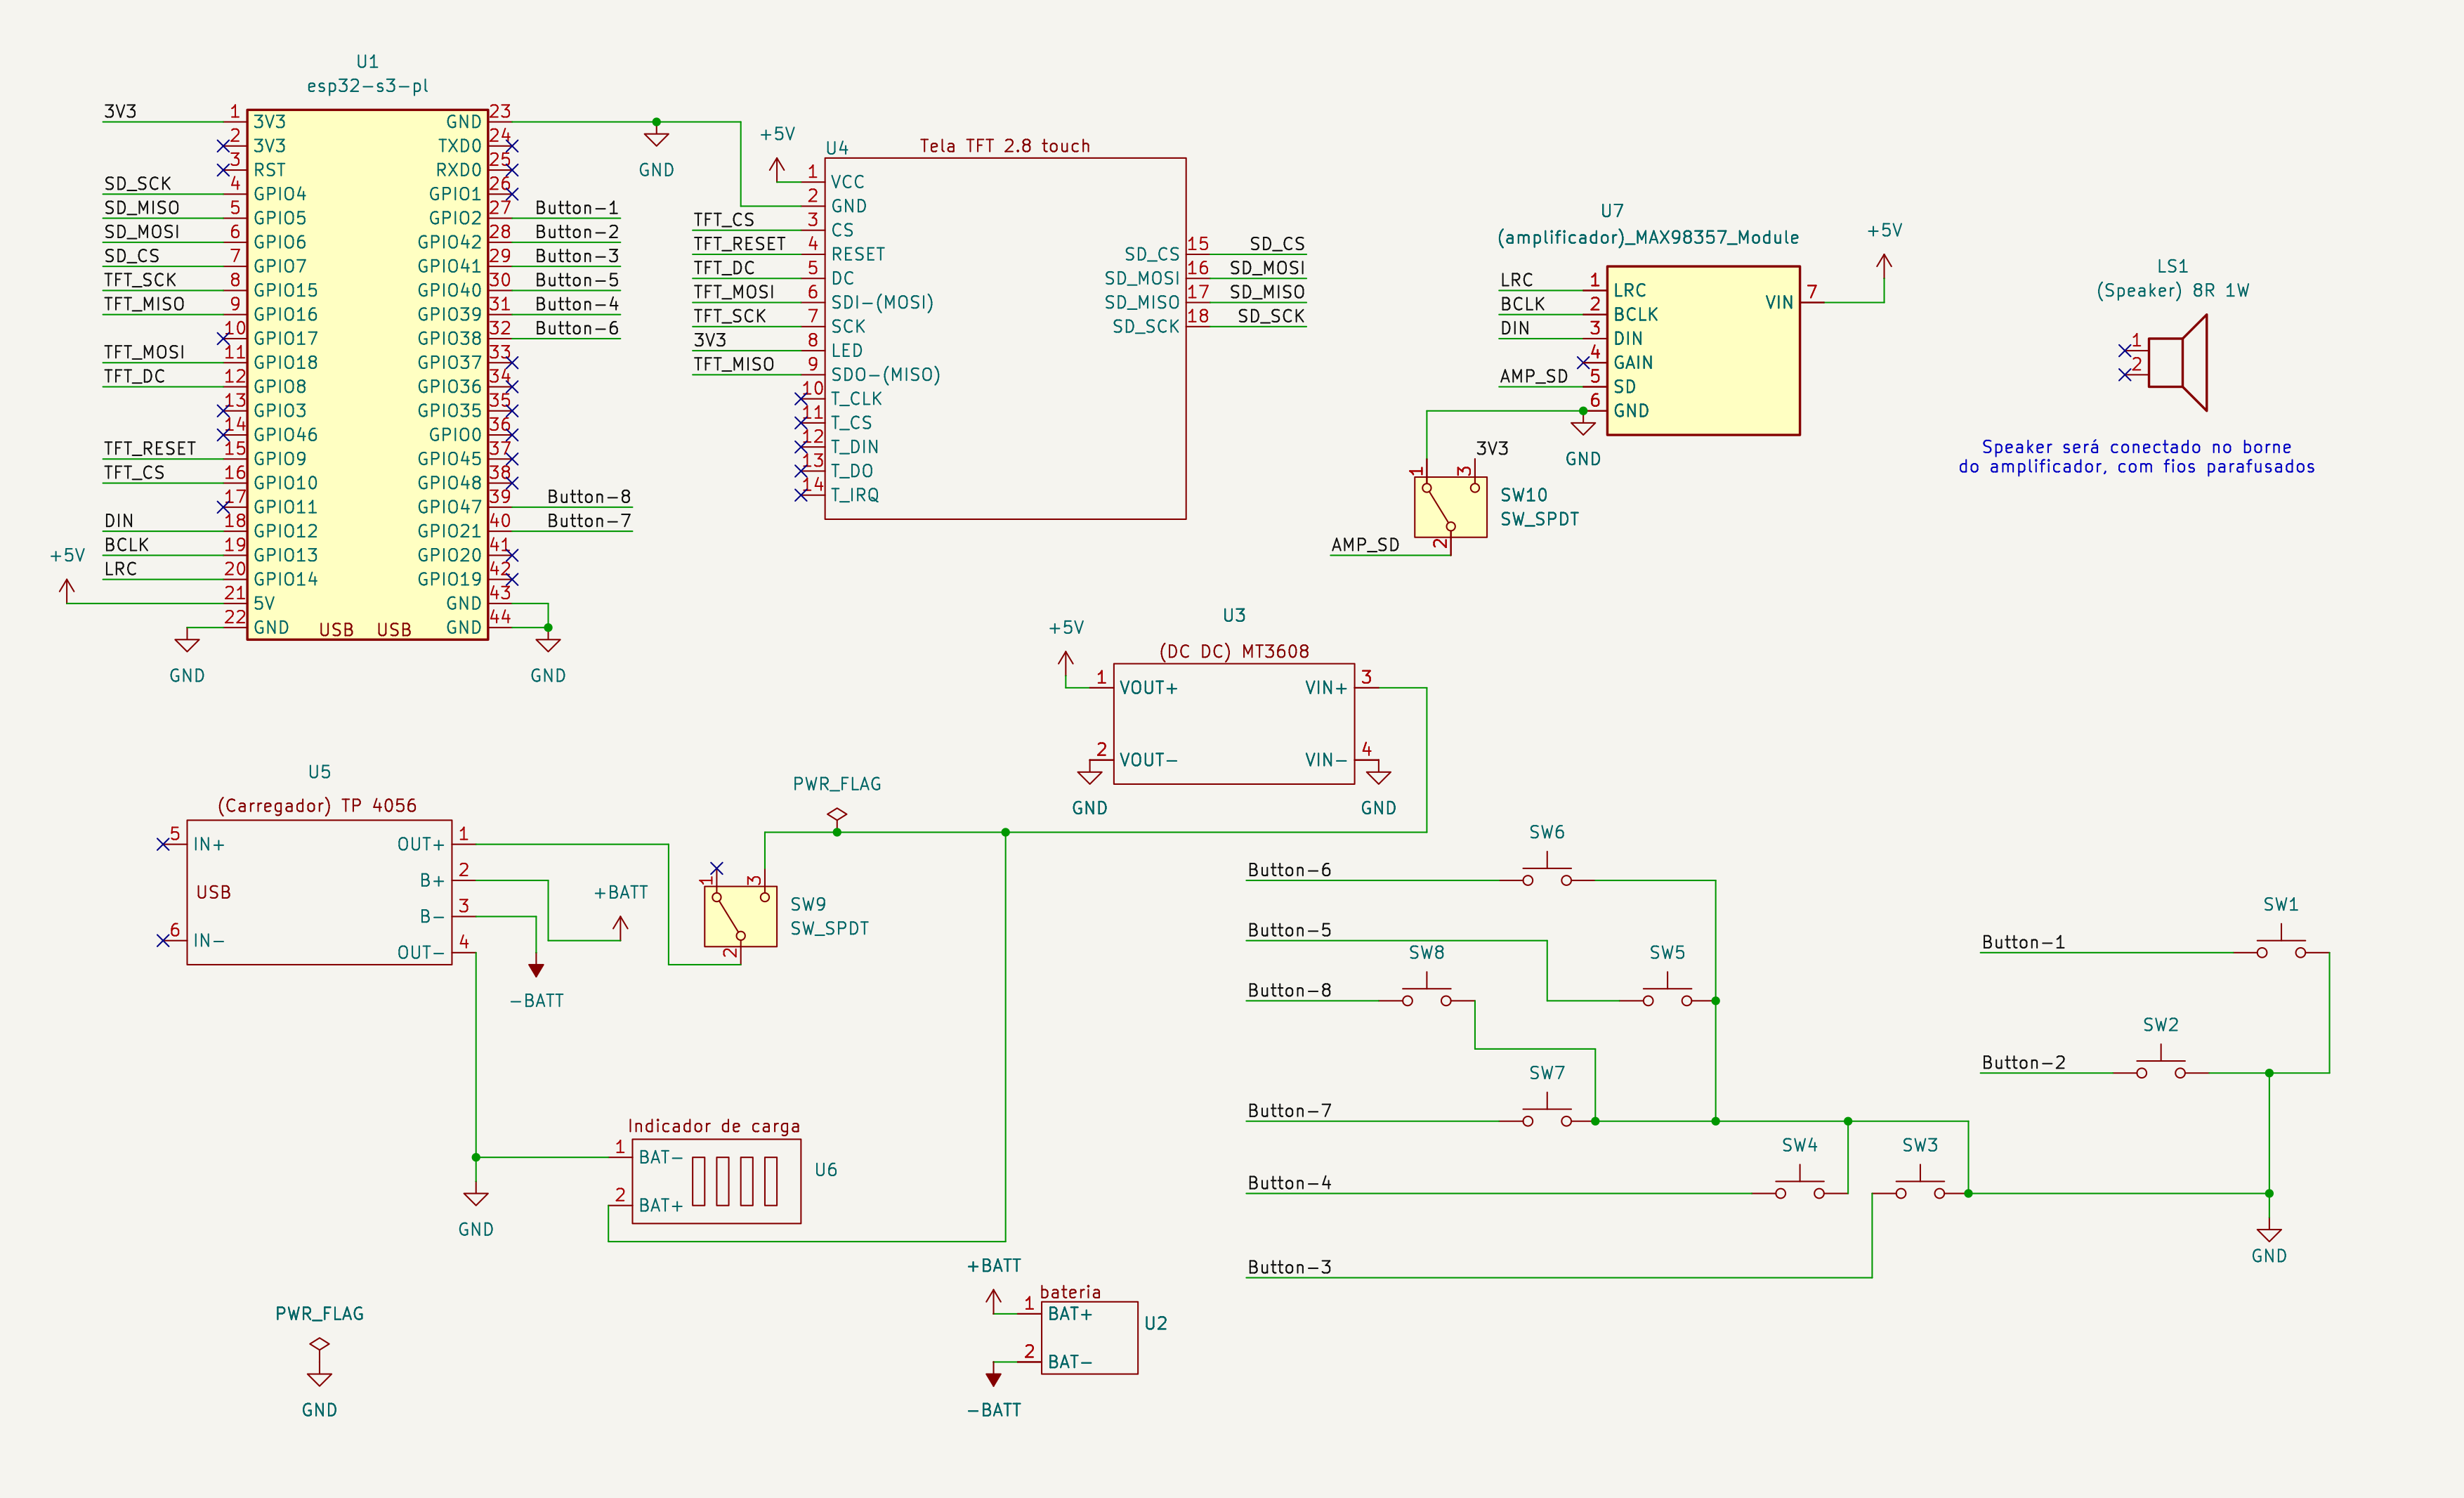
\includegraphics[width=\linewidth,height=0.78\textwidth,keepaspectratio]{images/esquematico.png}
    \par\small Esquemático do console com processamento, display, áudio, controles e alimentação.
  \end{center}
\end{landscape}
\end{document}
